\documentclass[10pt]{article}
\usepackage[utf8]{inputenc}
\usepackage[includehead, headheight=10mm, margin=15mm ]{geometry}
\usepackage{amsmath}
\usepackage{amsthm}
\usepackage{amsfonts}
\usepackage{xcolor}
\usepackage{graphicx}
\usepackage{titling}
\usepackage{fancyhdr}
\usepackage{listings}

\title{APPM 4600 Homework 10}
\author{Edward Wawrzynek}
\date{8 November 2024}

\newcommand*{\dif}{\mathop{}\!\mathrm{d}}

\makeatletter
\def\@maketitle{%
  \newpage
  \null
  \vskip 1em%
  \begin{center}%
  \let \footnote \thanks
    {\LARGE \@title \par}%
    \vskip 1em%
    {\normalfont \@date}
  \end{center}%
  \par
  \vskip 1em}
\makeatother

\begin{document}

\pagestyle{fancy}
    \fancyhf{} % clear all header and footer fields
    \fancyhead[L]{\thetitle}
    \fancyhead[R]{\theauthor}

\makeatletter
\begin{center}
    {\Large \@title}
    \vskip 1mm
    {\normalfont \@date}
    \vskip 1em
\end{center}
\makeatother

\begin{enumerate}
    \item We wish to approximate \(f(x)\) with the rational approximation \begin{align*}
        f(x) = \frac{p(x)}{q(x)} = \frac{a_0 + a_1x + a_2x^2 + \dots + a_mx^m}{1 + b_1x + b_2x^2 + \dots + b_nx^n},
    \end{align*} where \(p\) is of degree \(m\) and \(q\) of degree \(n\). We take the Taylor expansion of \(f\) to degree \(m+n\), \begin{align*}
        f(x) \approx \mathbb{T}_{n+m}(x) = c_0 + c_1x + c_2x^2 + \dots + c_{n+m}x^{n+m},
    \end{align*} and have \begin{align}\label{eq:expand}
      \mathbb{T}_{n+m}(x)q(x) = p(x),
    \end{align} where we can match the terms on both sides up through order \(n+m\).

    We take the Taylor expansion of \(f(x) = \sin(x)\) about \(x=0\), \begin{align*}
        \mathbb{T}_{6} = x - \frac{1}{6}x^3 + \frac{1}{120}x^5.
    \end{align*}

    \begin{enumerate}
      \item We have \(m=n=3\), so \eqref{eq:expand} becomes \begin{align*}
        \left( x - \frac{1}{6}x^3 + \frac{1}{120}x^5 \right) \left(1 + b_1x + b_2x^2 + b_3x^3\right)  = a_0 + a_1x + a_2x^2 + a_3x^3,
      \end{align*} which gives the system \begin{align*}
        a_0 &= 0 \\
        a_1 &= 1 \\
        a_2 &= b_1 \\
        a_3 &= -\frac{1}{6} + b_2 \\
        0   &= b_3 - \frac{1}{6}b_1 \\
        0   &= -\frac{1}{6}b_2 + \frac{1}{120} \\
        0   &= -\frac{1}{6}b_3 + \frac{1}{120}b_1
      \end{align*} with solution \begin{align*}
        a_0 = 0, a_1=1, a_2=0, a_3=-\frac{7}{60}, b_1=0, b_2=\frac{1}{20}, b_3=0,
      \end{align*} which gives approximation \begin{align*}
          f(x) \approx \frac{x - \frac{7}{60}x^3}{1+\frac{1}{20}x^2}.
      \end{align*}

      \item We have \(m=2\), \(n=4\), \eqref{eq:expand} becomes \begin{align*}
        \left( x - \frac{1}{6}x^3 + \frac{1}{120}x^5 \right) \left(1 + b_1x + b_2x^2 + b_3x^3 + b_4x^4\right)  = a_0 + a_1x + a_2x^2,
      \end{align*} which gives the system \begin{align*}
          a_0 &= 0 \\
          a_1 &= 1 \\
          a_2 &= b_1 \\
          0   &= -\frac{1}{6} + b_2 \\
          0   &= -\frac{1}{6}b_1 + b_3 \\
          0   &= \frac{1}{120} -\frac{1}{6}b_2 + b_4 \\
          0   &= -\frac{1}{6}b_3 + \frac{1}{120}b_1,
      \end{align*} which has solution \begin{align*}
          a_0 = 0, a_1=1, a_2=0, b_1=0, b_2=\frac{1}{6}, b_3=0, b_4=\frac{7}{360},
      \end{align*} which gives the approximation \begin{align*}
          f(x) \approx \frac{x}{1+\frac{1}{6}x^2 + \frac{7}{360}x^4}
      \end{align*}

      \item We have \(m=4\), \(n=2\), so \eqref{eq:expand} becomes \begin{align*}
        \left( x - \frac{1}{6}x^3 + \frac{1}{120}x^5 \right) \left(1 + b_1x + b_2x^2\right)  = a_0 + a_1x + a_2x^2 + a_3x^3 + a_4x^4,
      \end{align*} which gives the system \begin{align*}
          a_0 &= 0 \\
          a_1 &= 1 \\
          a_2 &= b_1 \\
          a_3 &= -\frac{1}{6} + b_2 \\
          a_4 &= -\frac{1}{6}b_1 \\
          0   &= -\frac{1}{6}b_2 + \frac{1}{120} \\
          0   &= \frac{1}{120}b_1,
      \end{align*} with solution \begin{align*}
          a_0 = 0, a_1=1, a_2=0, a_3=\frac{7}{60}, a_4=0, b_1=0, b_2=\frac{1}{20},
      \end{align*} which gives approximation \begin{align*}
          f(x) \approx \frac{x-\frac{7}{60}x^3}{1+\frac{1}{20}x^2}.
      \end{align*}

      The error in these approximations versus the Taylor polynomial is plotted below. Notice that both parts (a) and (c) yielded the same rational approximations. The code used to generate these plots is listed below.

      \begin{center}
        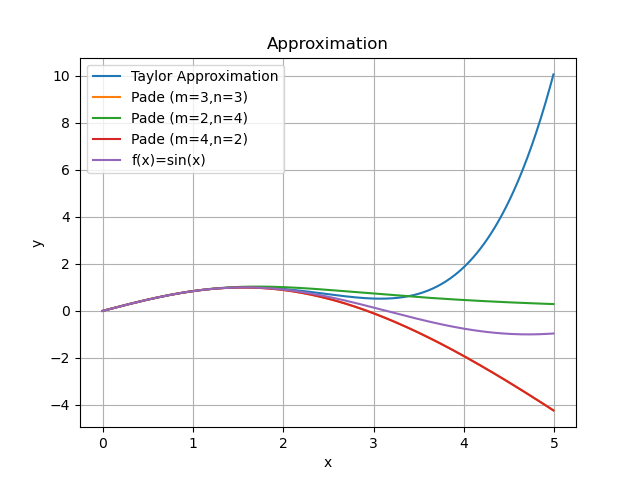
\includegraphics[width=0.45\textwidth]{pade.png}
        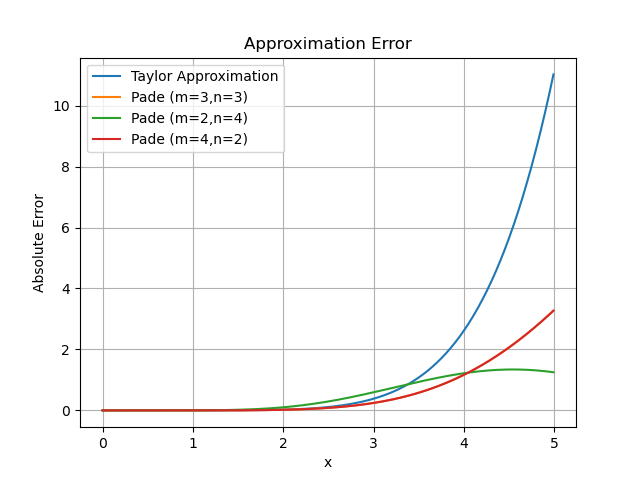
\includegraphics[width=0.45\textwidth]{pade_error.png}
      \end{center}
    \end{enumerate}

    {\small \lstinputlisting[language=Python]{hw10_1.py}}

    \item We have the quadrature \begin{align*}
        \int_0^1 f(x)\dif x = \frac{1}{2}f(x_0) + cf(x_1).
    \end{align*} We wish to be able to exactly integrate to 2 degree, which gives the system \begin{align*}
        \int_0^1 1 \dif x = 1 &= \frac{1}{2} + c, \\
        \int_0^1 x \dif x = \frac{1}{2} &= \frac{1}{2}x_0 + cx_1, \\
        \int_0^1 x^2 \dif x = \frac{1}{3} &= \frac{1}{2}x_0^2 + cx_1^2. \\
    \end{align*} The first equation gives \(c=\frac{1}{2}\). The last two are nonlinear, and can be rearranged to give \begin{align*}
        x_1 &= 1 - x_0, \\
        \frac{2}{3} &= x_0^2 + (1-x_0)^2 = 2x_0^2 -2x_0 + 1, 
    \end{align*} which implies \begin{align*}
        0 = 6x_0^2 - 6x_0 + 1,
    \end{align*} which has solutions \begin{align*}
        x_0 = \frac{3 \pm \sqrt{3}}{6}, x_1 &= \frac{3 \mp \sqrt{3}}{6}.
    \end{align*} Without loss of generality, we pick \(x_0 = \frac{3 - \sqrt{3}}{6}\) and \(x_1 = \frac{3 + \sqrt{3}}{6}\), and have the quadrate \begin{align*}
      \int_0^1 f(x)\dif x = \frac{1}{2}f\left(\frac{3 - \sqrt{3}}{6}\right) + \frac{1}{2}f\left(\frac{3 + \sqrt{3}}{6}\right).
    \end{align*}

\end{enumerate}


\end{document}
